%\setcounter{chapter}{1}
\chapter{Luyện tập: Lực Lo-ren-xơ}
\section{Tính các đại lượng trong công thức lực Lo-ren-xơ}
\begin{enumerate}
	\item  Cho electron bay vào miền có từ trường đều với vận tốc $v = 8\cdot 10^5\ \text{m/s}$ theo phương vuông góc với vectơ cảm ứng từ, độ lớn cảm úng từ là $B = \text{9,1}\cdot 10^{-4}\ \text{T}$. Tính độ lớn lực Lo-ren-xơ tác dụng lên electron.
	\begin{mcq}(4)
		\item $\text{1,1648}\cdot 10^{-16}\ \text{N}$.
		\item $\text{1,1648}\cdot 10^{-17}\ \text{N}$.
		\item $\text{1,1648}\cdot 10^{-19}\ \text{N}$.
		\item $\text{1,1648}\cdot 10^{-20}\ \text{N}$.
	\end{mcq}
	
	\item Một hạt mang điện $\text{3,2}\cdot 10^{-19}\ \text{C}$ bay vào trong từ trường đều có $B = \text{0,5}\ \text{T}$ hợp với hướng của đường sức từ $30^\circ$. Lực Lorenxơ tác dụng lên hạt có độ lớn $\text{8}\cdot 10^{-14}\ \text{N}$. Vận tốc của hạt đó khi bắt đầu vào trong từ trường là bao nhiêu?
	\begin{mcq}(4)
		\item $v = 2\cdot 10^6\ \text{m/s}$.
		\item $v = \cdot 10^6\ \text{m/s}$.
		\item $v = 3\cdot 10^6\ \text{m/s}$.
		\item $v = 5\cdot 10^6\ \text{m/s}$.
	\end{mcq}
	
	\item  Một hạt điện tích chuyên động trong từ trường đều quĩ đạo của hạt vuông góc với đường sức từ. Nếu hạt chuyển động với vận tốc $v_1=\text{1,8}\cdot 10^{6}\ \text{m/s}$ thì lực Lo-ren-xơ tác dụng lên hạt có độ lớn là $f_1=\text{2}\cdot 10^{-6}\ \text{N}$, nêu hạt chuyển động với vận tốc là $v_1=\text{4,5}\cdot 10^{7}\ \text{m/s}$ thì lực Loren tác dụng lên hạt có giá trị là
	\begin{mcq}(2)
		\item $f_2=\text{2}\cdot 10^{-5}\ \text{N}$.
		\item $f_2=\text{3}\cdot 10^{-5}\ \text{N}$.
		\item $f_2=\text{5}\cdot 10^{-5}\ \text{N}$.
		\item $f_2=\text{6}\cdot 10^{-5}\ \text{N}$.
	\end{mcq}
\end{enumerate}

\section{Xác định phương, chiều lực Lo-ren-xơ}
\begin{enumerate}
	\item Trong hình vẽ sau hình nào chỉ đúng hướng của lực Lorenxơ tác dụng lên hạt mang điện dương chuyển động trong từ trường đều?
	\begin{mcq}(2)
		\item 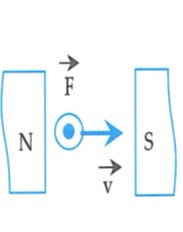
\includegraphics[scale=0.8]{../figs/VN11-PH-27-P-018-1-h1.jpg}
		\item 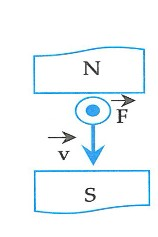
\includegraphics[scale=0.8]{../figs/VN11-PH-27-P-018-1-h2.jpg}
		\item 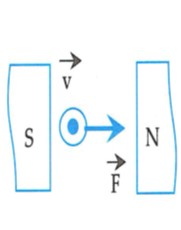
\includegraphics[scale=0.8]{../figs/VN11-PH-27-P-018-1-h3.jpg}
		\item 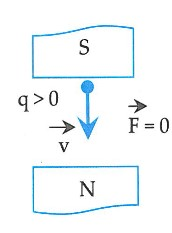
\includegraphics[scale=0.8]{../figs/VN11-PH-27-P-018-1-h4.jpg}
	\end{mcq}
	
	\item Trong hình vẽ sau hình nào chỉ đúng hướng của lực Lorenxơ tác dụng lên electron chuyển động trong từ trường đều?
	\begin{mcq}(2)
		\item 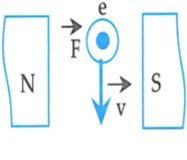
\includegraphics[scale=0.8]{../figs/VN11-PH-27-P-018-1-h5.jpg}
		\item 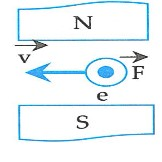
\includegraphics[scale=0.8]{../figs/VN11-PH-27-P-018-1-h6.jpg}
		\item 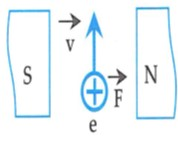
\includegraphics[scale=0.8]{../figs/VN11-PH-27-P-018-1-h7.jpg}
		\item 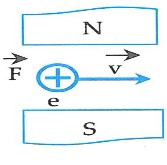
\includegraphics[scale=0.8]{../figs/VN11-PH-27-P-018-1-h8.jpg}
	\end{mcq}
	
	\item Trong hình vẽ sau hình nào chỉ đúng hướng của lực Lorenxơ tác dụng lên electron và hạt mang điện dương chuyển động trong từ trường đều?
	\begin{mcq} (2)
		\item 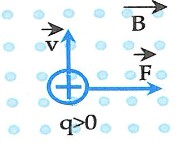
\includegraphics[scale=0.8]{../figs/VN11-PH-27-P-018-1-h9.jpg}
		\item 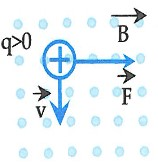
\includegraphics[scale=0.8]{../figs/VN11-PH-27-P-018-1-h10.jpg}
		\item 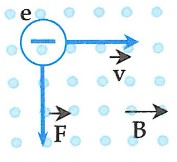
\includegraphics[scale=0.8]{../figs/VN11-PH-27-P-018-1-h11.jpg}
		\item 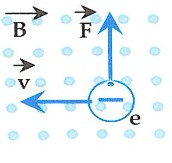
\includegraphics[scale=0.8]{../figs/VN11-PH-27-P-018-1-h12.jpg}
	\end{mcq}
	
	\item  Trong hình vẽ sau hình nào chỉ đúng hướng của lực Lorenxơ tác dụng lên electron chuyển động trong từ trường đều?
	\begin{mcq}(2)
		\item 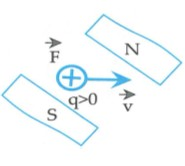
\includegraphics[scale=0.8]{../figs/VN11-PH-27-P-018-1-h13.jpg}
		\item 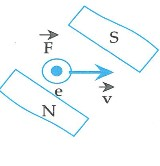
\includegraphics[scale=0.8]{../figs/VN11-PH-27-P-018-1-h14.jpg}
		\item 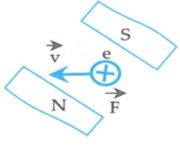
\includegraphics[scale=0.8]{../figs/VN11-PH-27-P-018-1-h15.jpg}
		\item 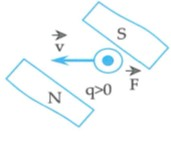
\includegraphics[scale=0.8]{../figs/VN11-PH-27-P-018-1-h16.jpg}
	\end{mcq}
	
	
\end{enumerate}
\section{Chuyển động của hạt mang điện trong từ trường đều}
\begin{enumerate}
	\item  Hạt electron với vận tốc đầu bằng không được gia tốc qua một hiệu điện thế 400 V. Tiếp đó nó được dẫn vào miền có từ trường đều vuông góc hướng chuyển động. Quỹ đạo của electron là đường tròn bán kính $R = 7\ \text{cm}$. Xác định độ lớn cảm ứng từ $B$.
	\begin{mcq}(4)
		\item $\text{9,636}\cdot 10^{-4}\ \text{T}$.
		\item $\text{4,818}\cdot 10^{-4}\ \text{T}$.
		\item $\text{3,212}\cdot 10^{-4}\ \text{T}$.
		\item $\text{6,242}\cdot 10^{-4}\ \text{T}$.
	\end{mcq}
	
	\item Một ion bay theo quỹ đạo hòn bán kính $R$ trong một mặt phăng vuông góc với các đường sức của một từ trường đều. Khi độ lớn vận tốc tăng gấp đôi thì bán kính quỹ đạo là 
	\begin{mcq}(4)
		\item $\dfrac{R}{2}.$
		\item $\dfrac{R}{4}.$
		\item $2R.$
		\item $4R.$
	\end{mcq}
\end{enumerate}	

\begin{center}
	\textbf{ĐÁP ÁN}
	
\end{center}




\textbf{1. Tính các đại lượng trong công thức lực Lo-ren-xơ}

\begin{longtable}[\textwidth]{|p{0.1\textwidth}|p{0.1\textwidth}|p{0.1\textwidth}|p{0.1\textwidth}|p{0.1\textwidth}|p{0.1\textwidth}|p{0.1\textwidth}|p{0.1\textwidth}|}
	% --- first head
	\hline%\hspace{2 pt}
	\multicolumn{1}{|c}{\textbf{Câu 1}} & \multicolumn{1}{|c|}{\textbf{Câu 2}} & \multicolumn{1}{c|}{\textbf{Câu 3}} &
	\multicolumn{1}{c|}{\textbf{}} &
	\multicolumn{1}{c|}{\textbf{}} &
	\multicolumn{1}{c|}{\textbf{}} &
	\multicolumn{1}{c|}{\textbf{}} &
	\multicolumn{1}{c|}{\textbf{}}\\
	\hline
	A.&B. &C. & & & & &	\\
	\hline
	
	
\end{longtable}


\textbf{2. Xác định phương, chiều lực Lo-ren-xơ}

\begin{longtable}[\textwidth]{|p{0.1\textwidth}|p{0.1\textwidth}|p{0.1\textwidth}|p{0.1\textwidth}|p{0.1\textwidth}|p{0.1\textwidth}|p{0.1\textwidth}|p{0.1\textwidth}|}
	% --- first head
	\hline%\hspace{2 pt}
	\multicolumn{1}{|c}{\textbf{Câu 1}} & \multicolumn{1}{|c|}{\textbf{Câu 2}} & \multicolumn{1}{c|}{\textbf{Câu 3}} &
	\multicolumn{1}{c|}{\textbf{Câu 4}} &
	\multicolumn{1}{c|}{\textbf{}} &
	\multicolumn{1}{c|}{\textbf{}} &
	\multicolumn{1}{c|}{\textbf{}} &
	\multicolumn{1}{c|}{\textbf{}}\\
	\hline
	D.&C. &A. &A. & & & &	\\
	\hline
\end{longtable}

\textbf{3. Chuyển động của hạt mang điện trong từ trường đều}

\begin{longtable}[\textwidth]{|p{0.1\textwidth}|p{0.1\textwidth}|p{0.1\textwidth}|p{0.1\textwidth}|p{0.1\textwidth}|p{0.1\textwidth}|p{0.1\textwidth}|p{0.1\textwidth}|}
	% --- first head
	\hline%\hspace{2 pt}
	\multicolumn{1}{|c}{\textbf{Câu 1}} & \multicolumn{1}{|c|}{\textbf{Câu 2}} & \multicolumn{1}{c|}{\textbf{}} &
	\multicolumn{1}{c|}{\textbf{}} &
	\multicolumn{1}{c|}{\textbf{}} &
	\multicolumn{1}{c|}{\textbf{}} &
	\multicolumn{1}{c|}{\textbf{}} &
	\multicolumn{1}{c|}{\textbf{}}\\
	\hline
	A.&C. & & & & & &	\\
	\hline
\end{longtable}










